\documentclass{../../ece-report}

\usepackage{subcaption}
\usepackage{circuitikz}
\usepackage{subcaption}

\newcommand{\twosubfigures}[6]{
  \begin{subfigure}{0.45\textwidth}
    \includegraphics[width=\textwidth]{#1}
    \caption{#2}
    \label{#3}
  \end{subfigure}
  \begin{subfigure}{0.45\textwidth}
    \includegraphics[width=\textwidth]{#4}
    \caption{#5}
    \label{#6}
  \end{subfigure}
}


\memostudent{Ty Davis}
\memotitle{Lab 4 - MOSFET Operation}
\memocourse{ECE 3110}
\memodate{\today}

\begin{document}

\maketitle

\section{Introduction and Theory}

In this lab we are measuring the characteristics
of operation of a MOSFET, specifically the 2N2700. The circuit that we build
is shown in Fig.~\ref{fig:circuit}.

\begin{figure}[h!]
  \centering
  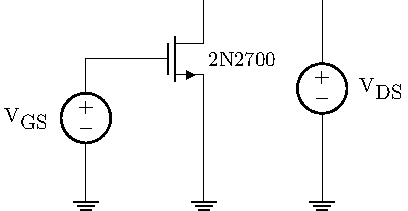
\includegraphics{circuits/circuit.pdf}
  \caption{Circuit for the Lab.}
  \label{fig:circuit}
\end{figure}

MOSFET's operate in different conditions depending on
the relative voltages V$_{GS}$ and V$_{DS}$. Depending
on the difference of those voltages the MOSFET might
be in what's called the \emph{triode} or \emph{saturation}
region.

In order to find $k_n$ we can use the following two expressions.

\[
  k_n = k_n'\Big( \frac{W}{L} \Big)
\]

\[
  i_D = \frac{1}{2} k_n'\Big( \frac{W}{L} \Big) V_{OV}^2
\]

Combining those we get Eq.~\ref{eq:kn}.

\begin{equation}
  k_n = \frac{2 i_D}{V_{OV}^2}
  \label{eq:kn}
\end{equation}

\section{Results}

In Fig.~\ref{fig:sweep_vgs}  you can see the V$_{GS}$
voltage where the graph starts to increase dramatically,
and it appears to be right at the same spot when we
measured it. This is our threshold voltage: V$_{T} =
2.0$~V.

Using Eq.~\ref{eq:kn}, the average calculated $k_n$
for the simulations was $k_n = 0.096~\si{\A}/\si{\V^2}$,
and the average calculated $k_n$ for the measurements
was $k_n = 0.155~\si{\A}/\si{\V^2}$. The values for
$i_D$ and $V_{OV}$ that were used for the calculation
are shown in Fig.~\ref{fig:sweep_vds}.



\begin{figure}
  \centering
  \twosubfigures{../plots/pdf/sim_sweep_vgs.pdf}{Simulated}{fig:vgs_simulated}
                {../plots/pdf/sweep_vgs.pdf}{Measured}{fig:vgs_measured}
  \caption{Sweep V$_{GS}$}
  \label{fig:sweep_vgs}
\end{figure}

\begin{figure}
  \centering
  \twosubfigures{../plots/pdf/sim_sweep_vds.pdf}{Simulated}{fig:vds_simulated}
                {../plots/pdf/sweep_vds.pdf}{Measured}{fig:vds_measured}
  \caption{Sweep V$_{DS}$}
  \label{fig:sweep_vds}
\end{figure}

\begin{table}[h!]
  \centering
  \begin{tabular}[c]{ll}
    \multicolumn{1}{c}{\textbf{V$_{GS}$}} & 
    \multicolumn{1}{c}{\textbf{V$_A$}} \\
    \hline
    2.5 V & -4970.8 V \\
    3.0 V & -1099.6 V \\
    3.5 V & -6426.9 V \\
    \hline
    \textbf{Avg} & -4165.7 V \\
  \end{tabular}
  \caption{Early Voltages calculated from the simulation.}
  \label{tab:early_sim}
\end{table}


\begin{table}[h!]
  \centering
  \begin{tabular}[c]{ll}
    \multicolumn{1}{c}{\textbf{V$_{GS}$}} & 
    \multicolumn{1}{c}{\textbf{V$_A$}} \\
    \hline
    2.5 V & -6.07 V \\
    3.0 V & -3.12 V \\
    \hline
    \textbf{Avg}   & -4.60 V \\
  \end{tabular}
  \caption{Early Voltages calculated from the measurement.}
  \label{tab:early_meas}
\end{table}

Table~\ref{tab:early_sim} shows the Early voltages calculated
from the simulation results shown in Fig.~\ref{fig:vds_simulated}.
The average of those calculated Early voltages is V$_{A}
= -4165.7$~V for the simulation and V$_{A} = -4.60$~V for the measurements.

The $\lambda$ value is accordingly: $\lamba=-0.00024~1/\si{\V}$
for the simulation and $\lambda=-0.22~1/\si{\V}$ for
the measurements. Clearly those values don't exactly
line up between the simulation and the measurements.
This is likely because we couldn't get enough current
from the function generator to measure the appropriate
values of V$_{DS}$ and i$_D$.




\section{Conclusion}

This lab proved difficult because the multi-meters were
not cooperating, so we changed the circuit slightly
to obtain the values another way. We placed a resistor
between the V$_{DS}$ voltage supply and the drain connection
of the MOSFET so that we could measure the voltage across
it and in eventually calculate the current through the
drain of the MOSFET. As you can see in Fig.~\ref{fig:sweep_vds},
while this did work we weren't able to get enough current
from the function generator to drive the V$_{DS}$ high
enough and in turn calculate the entire curve.

If I were to do this lab again I would try to use a
simpler multi-meter that doesn't try to auto-adjust
according to its measurements. That would likely result
in a better and much simpler outcome.

\end{document}
